\pagebreak
\subsection{Sequence Diagram}

\paragraph[]{Sequence diagram for traditional product entity update.} \hspace{1mm} \par
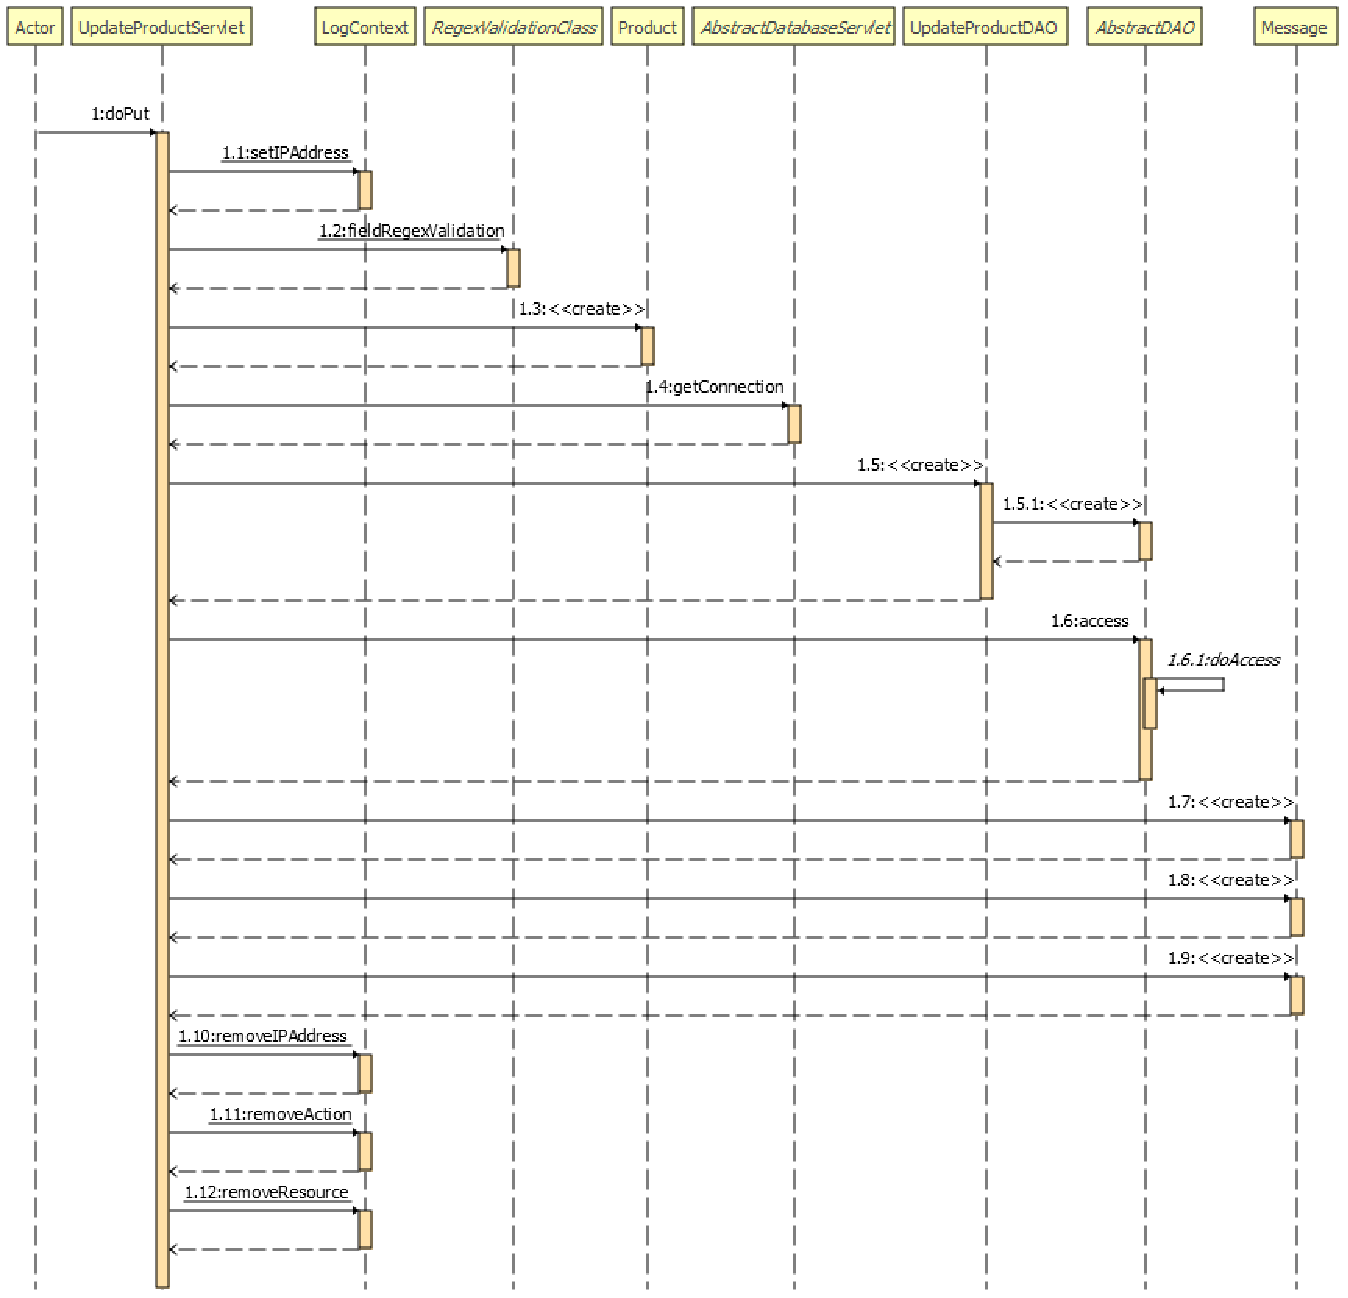
\includegraphics[width=\textwidth, keepaspectratio]{resources/updateproductsequence.pdf}
In the schema above is shown the sequence diagram for the update of a product. 

The user sends a PUT request to the web server. The web server calls the UpdateProductServlet and then sets the IP address of LogContext and also checks, using the class regex validation, that the parameters passed in input are valid.

Then a new object of class Product is created, with the parameters passed in input. After this, the UpdateProductServlet calls the getConection() method of the AbstractDatabaseServlet. After doing this, the servlet instantiate a new object of the class UpdateProductDAO, which extends AbstractDAO (so an object of AbstractDAO is created).

Then, with the doAccess() method of the class AbstractDAO, the DAO connects to the database.

After connecting to the database and executing the SQL statement, three messages for the servlet are created.

Finally, the resources are removed for the clean-up.
\pagebreak
\paragraph[]{Sequence diagram for rest get customer resource.} \hspace{1mm} \par
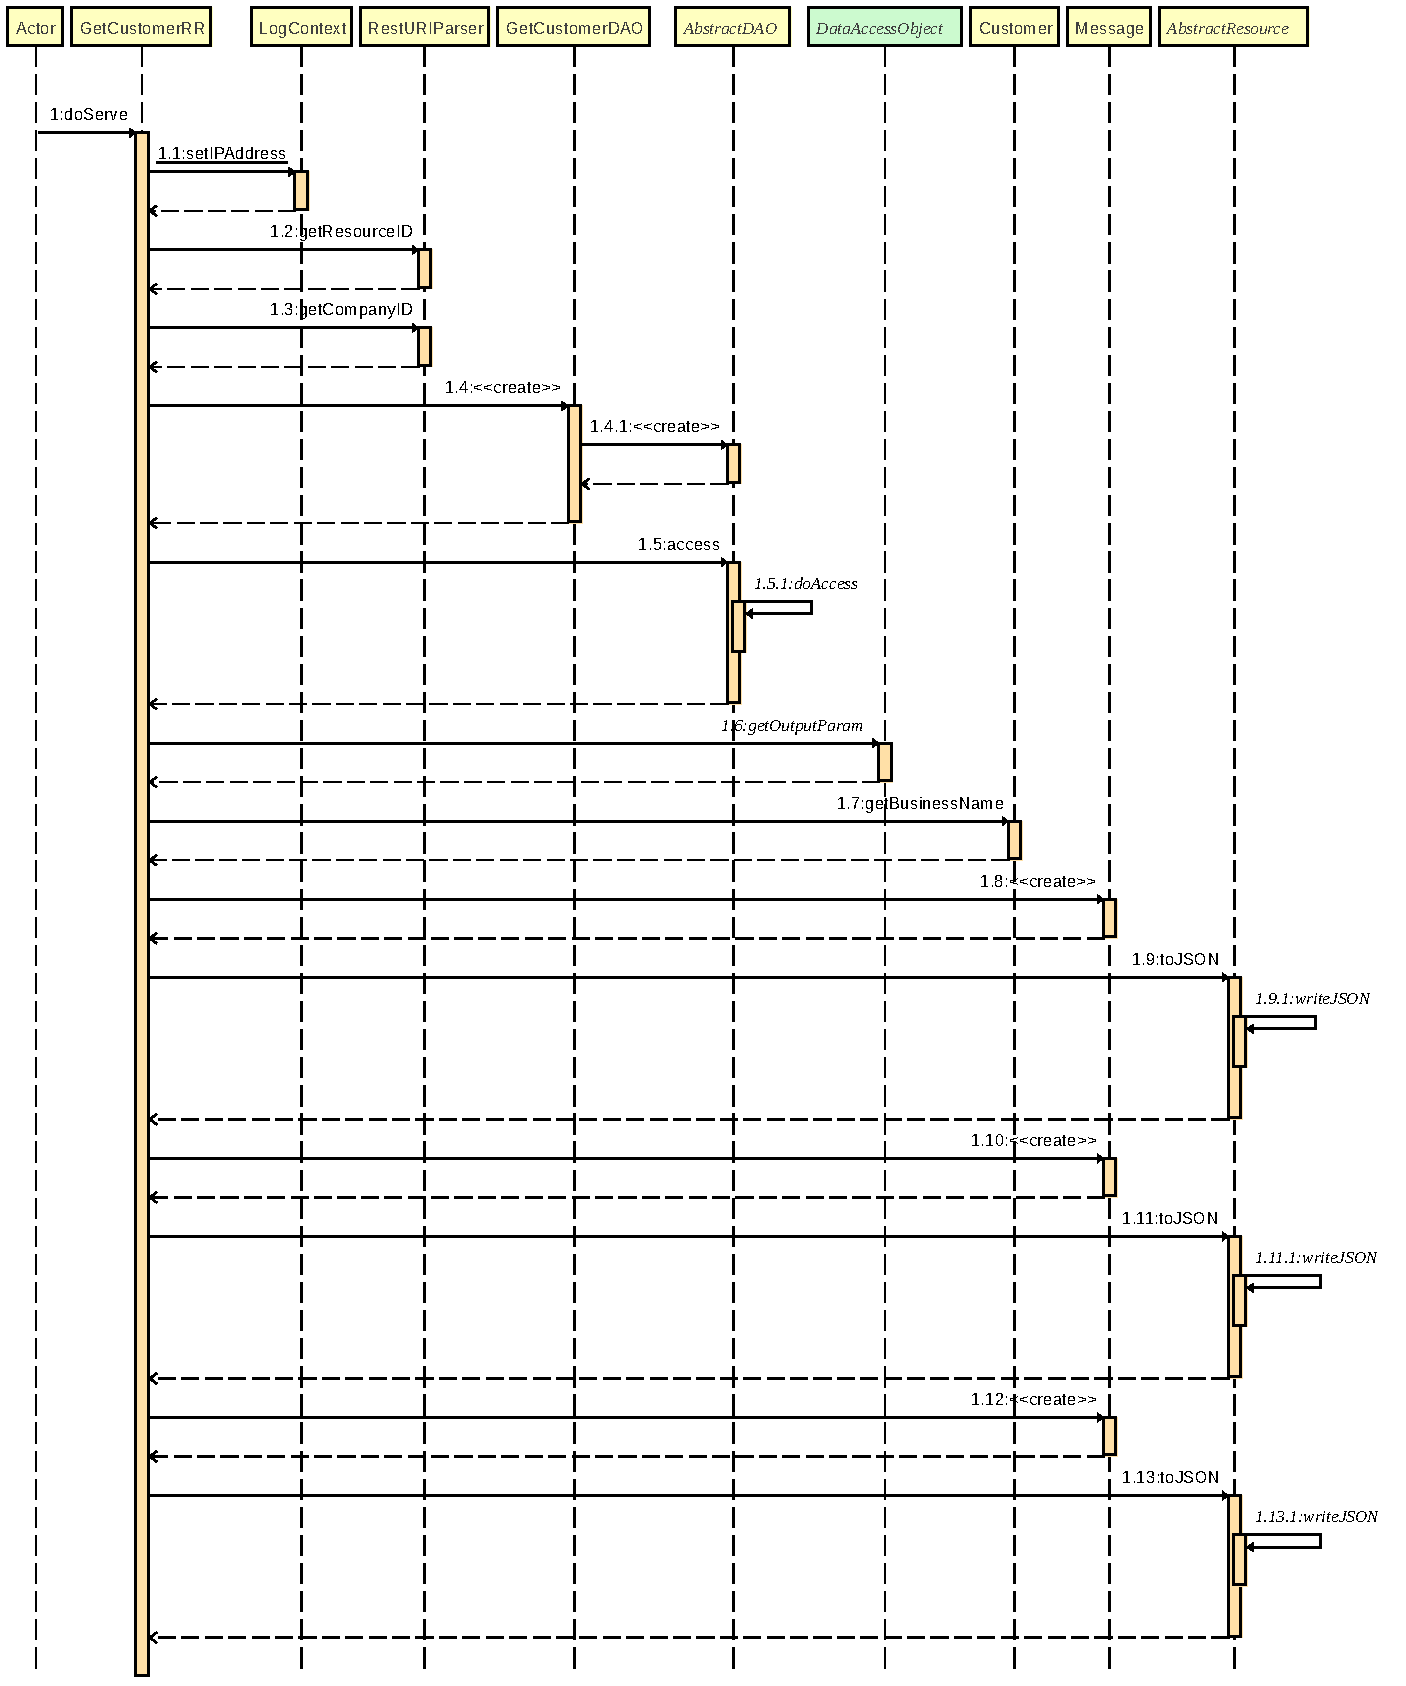
\includegraphics[width=\textwidth, keepaspectratio]{resources/getcustomersequence.pdf}


%describe here the sequence diagram